
%% bare_jrnl.tex
%% V1.4b
%% 2015/08/26
%% by Michael Shell
%% see http://www.michaelshell.org/
%% for current contact information.
%%
%% This is a skeleton file demonstrating the use of IEEEtran.cls
%% (requires IEEEtran.cls version 1.8b or later) with an IEEE
%% journal paper.
%%
%% Support sites:
%% http://www.michaelshell.org/tex/ieeetran/
%% http://www.ctan.org/pkg/ieeetran
%% and
%% http://www.ieee.org/

%%*************************************************************************
%% Legal Notice:
%% This code is offered as-is without any warranty either expressed or
%% implied; without even the implied warranty of MERCHANTABILITY or
%% FITNESS FOR A PARTICULAR PURPOSE! 
%% User assumes all risk.
%% In no event shall the IEEE or any contributor to this code be liable for
%% any damages or losses, including, but not limited to, incidental,
%% consequential, or any other damages, resulting from the use or misuse
%% of any information contained here.
%%
%% All comments are the opinions of their respective authors and are not
%% necessarily endorsed by the IEEE.
%%
%% This work is distributed under the LaTeX Project Public License (LPPL)
%% ( http://www.latex-project.org/ ) version 1.3, and may be freely used,
%% distributed and modified. A copy of the LPPL, version 1.3, is included
%% in the base LaTeX documentation of all distributions of LaTeX released
%% 2003/12/01 or later.
%% Retain all contribution notices and credits.
%% ** Modified files should be clearly indicated as such, including  **
%% ** renaming them and changing author support contact information. **
%%*************************************************************************


% *** Authors should verify (and, if needed, correct) their LaTeX system  ***
% *** with the testflow diagnostic prior to trusting their LaTeX platform ***
% *** with production work. The IEEE's font choices and paper sizes can   ***
% *** trigger bugs that do not appear when using other class files.       ***                          ***
% The testflow support page is at:
% http://www.michaelshell.org/tex/testflow/



\documentclass[journal]{IEEEtran}
%
% If IEEEtran.cls has not been installed into the LaTeX system files,
% manually specify the path to it like:
% \documentclass[journal]{../sty/IEEEtran}





% Some very useful LaTeX packages include:
% (uncomment the ones you want to load)


% *** MISC UTILITY PACKAGES ***
%
%\usepackage{ifpdf}
% Heiko Oberdiek's ifpdf.sty is very useful if you need conditional
% compilation based on whether the output is pdf or dvi.
% usage:
% \ifpdf
%   % pdf code
% \else
%   % dvi code
% \fi
% The latest version of ifpdf.sty can be obtained from:
% http://www.ctan.org/pkg/ifpdf
% Also, note that IEEEtran.cls V1.7 and later provides a builtin
% \ifCLASSINFOpdf conditional that works the same way.
% When switching from latex to pdflatex and vice-versa, the compiler may
% have to be run twice to clear warning/error messages.






% *** CITATION PACKAGES ***
%
\usepackage{cite}
% cite.sty was written by Donald Arseneau
% V1.6 and later of IEEEtran pre-defines the format of the cite.sty package
% \cite{} output to follow that of the IEEE. Loading the cite package will
% result in citation numbers being automatically sorted and properly
% "compressed/ranged". e.g., [1], [9], [2], [7], [5], [6] without using
% cite.sty will become [1], [2], [5]--[7], [9] using cite.sty. cite.sty's
% \cite will automatically add leading space, if needed. Use cite.sty's
% noadjust option (cite.sty V3.8 and later) if you want to turn this off
% such as if a citation ever needs to be enclosed in parenthesis.
% cite.sty is already installed on most LaTeX systems. Be sure and use
% version 5.0 (2009-03-20) and later if using hyperref.sty.
% The latest version can be obtained at:
% http://www.ctan.org/pkg/cite
% The documentation is contained in the cite.sty file itself.






% *** GRAPHICS RELATED PACKAGES ***
%
\ifCLASSINFOpdf
  \usepackage[pdftex]{graphicx}
  % declare the path(s) where your graphic files are
  \graphicspath{{./figures/}{../jpeg/}}
  % and their extensions so you won't have to specify these with
  % every instance of \includegraphics
  \DeclareGraphicsExtensions{.pdf,.jpeg,.png,.jpg}
\else
  % or other class option (dvipsone, dvipdf, if not using dvips). graphicx
  % will default to the driver specified in the system graphics.cfg if no
  % driver is specified.
   \usepackage[dvips]{graphicx}
  % declare the path(s) where your graphic files are
  % \graphicspath{{../eps/}}
  % and their extensions so you won't have to specify these with
  % every instance of \includegraphics
  % \DeclareGraphicsExtensions{.eps}
\fi

% graphicx was written by David Carlisle and Sebastian Rahtz. It is
% required if you want graphics, photos, etc. graphicx.sty is already
% installed on most LaTeX systems. The latest version and documentation
% can be obtained at: 
% http://www.ctan.org/pkg/graphicx
% Another good source of documentation is "Using Imported Graphics in
% LaTeX2e" by Keith Reckdahl which can be found at:
% http://www.ctan.org/pkg/epslatex
%
% latex, and pdflatex in dvi mode, support graphics in encapsulated
% postscript (.eps) format. pdflatex in pdf mode supports graphics
% in .pdf, .jpeg, .png and .mps (metapost) formats. Users should ensure
% that all non-photo figures use a vector format (.eps, .pdf, .mps) and
% not a bitmapped formats (.jpeg, .png). The IEEE frowns on bitmapped formats
% which can result in "jaggedy"/blurry rendering of lines and letters as
% well as large increases in file sizes.
%
% You can find documentation about the pdfTeX application at:
% http://www.tug.org/applications/pdftex





% *** MATH PACKAGES ***
%
\usepackage{amsmath}
% A popular package from the American Mathematical Society that provides
% many useful and powerful commands for dealing with mathematics.
%
% Note that the amsmath package sets \interdisplaylinepenalty to 10000
% thus preventing page breaks from occurring within multiline equations. Use:
%\interdisplaylinepenalty=2500
% after loading amsmath to restore such page breaks as IEEEtran.cls normally
% does. amsmath.sty is already installed on most LaTeX systems. The latest
% version and documentation can be obtained at:
% http://www.ctan.org/pkg/amsmath





% *** SPECIALIZED LIST PACKAGES ***
%
%\usepackage{algorithmic}
% algorithmic.sty was written by Peter Williams and Rogerio Brito.
% This package provides an algorithmic environment fo describing algorithms.
% You can use the algorithmic environment in-text or within a figure
% environment to provide for a floating algorithm. Do NOT use the algorithm
% floating environment provided by algorithm.sty (by the same authors) or
% algorithm2e.sty (by Christophe Fiorio) as the IEEE does not use dedicated
% algorithm float types and packages that provide these will not provide
% correct IEEE style captions. The latest version and documentation of
% algorithmic.sty can be obtained at:
% http://www.ctan.org/pkg/algorithms
% Also of interest may be the (relatively newer and more customizable)
% algorithmicx.sty package by Szasz Janos:
% http://www.ctan.org/pkg/algorithmicx




% *** ALIGNMENT PACKAGES ***
%
\usepackage{array}
% Frank Mittelbach's and David Carlisle's array.sty patches and improves
% the standard LaTeX2e array and tabular environments to provide better
% appearance and additional user controls. As the default LaTeX2e table
% generation code is lacking to the point of almost being broken with
% respect to the quality of the end results, all users are strongly
% advised to use an enhanced (at the very least that provided by array.sty)
% set of table tools. array.sty is already installed on most systems. The
% latest version and documentation can be obtained at:
% http://www.ctan.org/pkg/array


% IEEEtran contains the IEEEeqnarray family of commands that can be used to
% generate multiline equations as well as matrices, tables, etc., of high
% quality.




% *** SUBFIGURE PACKAGES ***
%\ifCLASSOPTIONcompsoc
%  \usepackage[caption=false,font=normalsize,labelfont=sf,textfont=sf]{subfig}
%\else
  \usepackage[caption=false,font=footnotesize]{subfig}
%\fi
% subfig.sty, written by Steven Douglas Cochran, is the modern replacement
% for subfigure.sty, the latter of which is no longer maintained and is
% incompatible with some LaTeX packages including fixltx2e. However,
% subfig.sty requires and automatically loads Axel Sommerfeldt's caption.sty
% which will override IEEEtran.cls' handling of captions and this will result
% in non-IEEE style figure/table captions. To prevent this problem, be sure
% and invoke subfig.sty's "caption=false" package option (available since
% subfig.sty version 1.3, 2005/06/28) as this is will preserve IEEEtran.cls
% handling of captions.
% Note that the Computer Society format requires a larger sans serif font
% than the serif footnote size font used in traditional IEEE formatting
% and thus the need to invoke different subfig.sty package options depending
% on whether compsoc mode has been enabled.
%
% The latest version and documentation of subfig.sty can be obtained at:
% http://www.ctan.org/pkg/subfig




% *** FLOAT PACKAGES ***
%
%\usepackage{fixltx2e}
% fixltx2e, the successor to the earlier fix2col.sty, was written by
% Frank Mittelbach and David Carlisle. This package corrects a few problems
% in the LaTeX2e kernel, the most notable of which is that in current
% LaTeX2e releases, the ordering of single and double column floats is not
% guaranteed to be preserved. Thus, an unpatched LaTeX2e can allow a
% single column figure to be placed prior to an earlier double column
% figure.
% Be aware that LaTeX2e kernels dated 2015 and later have fixltx2e.sty's
% corrections already built into the system in which case a warning will
% be issued if an attempt is made to load fixltx2e.sty as it is no longer
% needed.
% The latest version and documentation can be found at:
% http://www.ctan.org/pkg/fixltx2e


\usepackage{stfloats}
% stfloats.sty was written by Sigitas Tolusis. This package gives LaTeX2e
% the ability to do double column floats at the bottom of the page as well
% as the top. (e.g., "\begin{figure*}[!b]" is not normally possible in
% LaTeX2e). It also provides a command:
%\fnbelowfloat
% to enable the placement of footnotes below bottom floats (the standard
% LaTeX2e kernel puts them above bottom floats). This is an invasive package
% which rewrites many portions of the LaTeX2e float routines. It may not work
% with other packages that modify the LaTeX2e float routines. The latest
% version and documentation can be obtained at:
% http://www.ctan.org/pkg/stfloats
% Do not use the stfloats baselinefloat ability as the IEEE does not allow
% \baselineskip to stretch. Authors submitting work to the IEEE should note
% that the IEEE rarely uses double column equations and that authors should try
% to avoid such use. Do not be tempted to use the cuted.sty or midfloat.sty
% packages (also by Sigitas Tolusis) as the IEEE does not format its papers in
% such ways.
% Do not attempt to use stfloats with fixltx2e as they are incompatible.
% Instead, use Morten Hogholm'a dblfloatfix which combines the features
% of both fixltx2e and stfloats:
%
% \usepackage{dblfloatfix}
% The latest version can be found at:
% http://www.ctan.org/pkg/dblfloatfix




%\ifCLASSOPTIONcaptionsoff
%  \usepackage[nomarkers]{endfloat}
% \let\MYoriglatexcaption\caption
% \renewcommand{\caption}[2][\relax]{\MYoriglatexcaption[#2]{#2}}
%\fi
% endfloat.sty was written by James Darrell McCauley, Jeff Goldberg and 
% Axel Sommerfeldt. This package may be useful when used in conjunction with 
% IEEEtran.cls'  captionsoff option. Some IEEE journals/societies require that
% submissions have lists of figures/tables at the end of the paper and that
% figures/tables without any captions are placed on a page by themselves at
% the end of the document. If needed, the draftcls IEEEtran class option or
% \CLASSINPUTbaselinestretch interface can be used to increase the line
% spacing as well. Be sure and use the nomarkers option of endfloat to
% prevent endfloat from "marking" where the figures would have been placed
% in the text. The two hack lines of code above are a slight modification of
% that suggested by in the endfloat docs (section 8.4.1) to ensure that
% the full captions always appear in the list of figures/tables - even if
% the user used the short optional argument of \caption[]{}.
% IEEE papers do not typically make use of \caption[]'s optional argument,
% so this should not be an issue. A similar trick can be used to disable
% captions of packages such as subfig.sty that lack options to turn off
% the subcaptions:
% For subfig.sty:
% \let\MYorigsubfloat\subfloat
% \renewcommand{\subfloat}[2][\relax]{\MYorigsubfloat[]{#2}}
% However, the above trick will not work if both optional arguments of
% the \subfloat command are used. Furthermore, there needs to be a
% description of each subfigure *somewhere* and endfloat does not add
% subfigure captions to its list of figures. Thus, the best approach is to
% avoid the use of subfigure captions (many IEEE journals avoid them anyway)
% and instead reference/explain all the subfigures within the main caption.
% The latest version of endfloat.sty and its documentation can obtained at:
% http://www.ctan.org/pkg/endfloat
%
% The IEEEtran \ifCLASSOPTIONcaptionsoff conditional can also be used
% later in the document, say, to conditionally put the References on a 
% page by themselves.




% *** PDF, URL AND HYPERLINK PACKAGES ***
%
\usepackage{url}
% url.sty was written by Donald Arseneau. It provides better support for
% handling and breaking URLs. url.sty is already installed on most LaTeX
% systems. The latest version and documentation can be obtained at:
% http://www.ctan.org/pkg/url
% Basically, \url{my_url_here}.




% *** Do not adjust lengths that control margins, column widths, etc. ***
% *** Do not use packages that alter fonts (such as pslatex).         ***
% There should be no need to do such things with IEEEtran.cls V1.6 and later.
% (Unless specifically asked to do so by the journal or conference you plan
% to submit to, of course. )


% correct bad hyphenation here
\hyphenation{op-tical net-works semi-conduc-tor}


\begin{document}
%
% paper title
% Titles are generally capitalized except for words such as a, an, and, as,
% at, but, by, for, in, nor, of, on, or, the, to and up, which are usually
% not capitalized unless they are the first or last word of the title.
% Linebreaks \\ can be used within to get better formatting as desired.
% Do not put math or special symbols in the title.
\title{Detection of DCIS and IDC in Whole-Slide\\ H\&E Stained Breast Histopathology Images Using Stacked Convolutional Neural Networks}
%
%
% author names and IEEE memberships
% note positions of commas and nonbreaking spaces ( ~ ) LaTeX will not break
% a structure at a ~ so this keeps an author's name from being broken across
% two lines.
% use \thanks{} to gain access to the first footnote area
% a separate \thanks must be used for each paragraph as LaTeX2e's \thanks
% was not built to handle multiple paragraphs
%

\author{Guido~C.~A.~Zuidhof\textbf{*},
        Babak~Ehteshami~Bejnordi,
        Geert~Litjens,
        and~Jason~Farquhar% <-this % stops a space
\thanks{This paper was written as part of the master's thesis in Artificial Intelligence of G. C. A. Zuidhof. This project was supervised by B. Ehteshami Bejnordi, G. Litjens and J. Farquhar. \textit{Asterisk indicates corresponding author.}}% <-this % stops a space
\thanks{*G. C. A. Zuidhof is a student in the Artificial Intelligence Master's Programme at the Radboud University, 6525HP Nijmegen, The Netherlands (e-mail: guido.zuidhof@student.ru.nl).}% <-this % stops a space
\thanks{B. Ehteshami Bejnordi is with the Diagnostic Image Analysis Group, Radboud University Medical Center, 6500HB Nijmegen, The Netherlands.}%
\thanks{G. Litjens is with the Department of Pathology, Radboud University Medical Center, 6500HB Nijmegen,
The Netherlands.}%
\thanks{J. Farquhar is with the Department of Artificial Intelligence, Radboud University, 6525HP Nijmegen,
The Netherlands and the Donders Institute for Brain, Cognition and Behaviou, 6525EN Nijmegen, The Netherlands.}%

\thanks{First draft, work in progress; October 1, 2016.}}

% note the % following the last \IEEEmembership and also \thanks - 
% these prevent an unwanted space from occurring between the last author name
% and the end of the author line. i.e., if you had this:
% 
% \author{....lastname \thanks{...} \thanks{...} }
%                     ^------------^------------^----Do not want these spaces!
%
% a space would be appended to the last name and could cause every name on that
% line to be shifted left slightly. This is one of those "LaTeX things". For
% instance, "\textbf{A} \textbf{B}" will typeset as "A B" not "AB". To get
% "AB" then you have to do: "\textbf{A}\textbf{B}"
% \thanks is no different in this regard, so shield the last } of each \thanks
% that ends a line with a % and do not let a space in before the next \thanks.
% Spaces after \IEEEmembership other than the last one are OK (and needed) as
% you are supposed to have spaces between the names. For what it is worth,
% this is a minor point as most people would not even notice if the said evil
% space somehow managed to creep in.



% The paper headers
\markboth{IEEE Transactions on Medical Imaging,~Vol.~X, No.~X, October~2016}%
{Zuidhof \MakeLowercase{\textit{et al.}}: Automated detection and characterization of DCIS and IDC in Whole-Slide H\&E Stained Breast Histopathology Images}
% The only time the second header will appear is for the odd numbered pages
% after the title page when using the twoside option.
% 
% *** Note that you probably will NOT want to include the author's ***
% *** name in the headers of peer review papers.                   ***
% You can use \ifCLASSOPTIONpeerreview for conditional compilation here if
% you desire.




% If you want to put a publisher's ID mark on the page you can do it like
% this:
%\IEEEpubid{0000--0000/00\$00.00~\copyright~2015 IEEE}
% Remember, if you use this you must call \IEEEpubidadjcol in the second
% column for its text to clear the IEEEpubid mark.



% use for special paper notices
%\IEEEspecialpapernotice{(Invited Paper)}




% make the title area
\maketitle

% As a general rule, do not put math, special symbols or citations
% in the abstract or keywords.
\begin{abstract}
This paper presents and evaluates a method for detection and localization of breast malignant lesions in histopathological breast tissue images. The goal of this method is to best classify digitized whole-slide hematoxylin and eosin (H\&E) stained whole-slide images (WSIs) into three classes: benign, ductal carcinoma in situ (DCIS) and invasive ductal carcinoma (IDC). A convolutional neural network (CNN) was trained on small patches of these images, labeled with the class of the center pixel. To distinguish between the DCIS and IDC class the information available in these small patches is often not sufficient. A second CNN was trained on the output of the aforementioned network with a larger patch size to capture a larger context. Sliding this classifier across a whole slide image yields a probability map. From this probability map structural and statistical features were extracted, which were used to train a final classifier to predict the label for the whole-slide image. The system is evaluated on a dataset containing X WSIs of breast tissue using FROC analysis. The results show a...
\end{abstract}

% Note that keywords are not normally used for peerreview papers.
\begin{IEEEkeywords}
Computer-aided diagnosis, DCIS and IDC detection, deep learning, whole-slide imaging.
\end{IEEEkeywords}






% For peer review papers, you can put extra information on the cover
% page as needed:
% \ifCLASSOPTIONpeerreview
% \begin{center} \bfseries EDICS Category: 3-BBND \end{center}
% \fi
%
% For peerreview papers, this IEEEtran command inserts a page break and
% creates the second title. It will be ignored for other modes.
\IEEEpeerreviewmaketitle

%\begin{center} \bfseries \textsc{FIRST DRAFT} \end{center}

\section{Introduction}
% The very first letter is a 2 line initial drop letter followed
% by the rest of the first word in caps.
% 
% form to use if the first word consists of a single letter:
% \IEEEPARstart{A}{demo} file is ....
% 
% form to use if you need the single drop letter followed by
% normal text (unknown if ever used by the IEEE):
% \IEEEPARstart{A}{}demo file is ....
% 
% Some journals put the first two words in caps:
% \IEEEPARstart{T}{his demo} file is ....
% 
% Here we have the typical use of a "T" for an initial drop letter
% and "HIS" in caps to complete the first word.
\IEEEPARstart{B}{reast} cancer is the most common cancer in women~\cite{cancerstats}. Cancers of the breast kill more women than any other form of cancer in all parts of the developing world~\cite{bcstats}. An important tool for the detection and management of breast cancer is analysis of tissue samples under the microscope by a pathologist.

Looking at cancer cells under the microscope, the pathologist searches for certain features that can help predict how likely the cancer is to grow and spread. These features include the spatial arrangement of the cells, morphometric characteristics of the nuclei, whether they form tubules, and how many of the cancer cells are in the process of dividing (mitotic count). These features taken together determine the extent or spread of cancer at the time of diagnosis.

Increasingly, slides of human tissue are digitized instead of being analysed only under a microscope. This has spawned the relatively new field of \emph{digital pathology}. Digital images as opposed to glass slides allow for  easier consultations between pathology experts. An additional advantage of digital images is the opportunity to analyze these images automatically using computer algorithms.

Visual microscopic interpretation of tissue sections is laborious and prone to subjectivity. \emph{Computer-aided diagnosis (CAD)} has a huge potential in alleviating shortcomings of human interpretation and will reduce the workload of the pathologists. As a result, more accurate diagnostic information may be extracted, helping clinicians in selecting the most optimal treatment for individual patients. CAD can facilitate diagnosis by sieving out obviously benign slides and providing quantitative characterization of suspicious areas.


\subsection{Patch-based classification}

Convolutional neural networks, as well as other statistical machine learning methods, are bound by computational and memory constraints. The tissue slides are scanned at a high magnification (up to 40X), resulting in very large images. A typical image can be 100,000 by 200,000 pixels, and have a file size of around 20GB uncompressed. 

To create a classification for the whole-slide image a patch based method will be employed. A patch is a small sub-image of the whole image. By applying the classifier in a sliding window approach over the original image we can create a prediction map for the whole image.

\begin{figure*}[!t]
\centering
\hspace{-0.1in}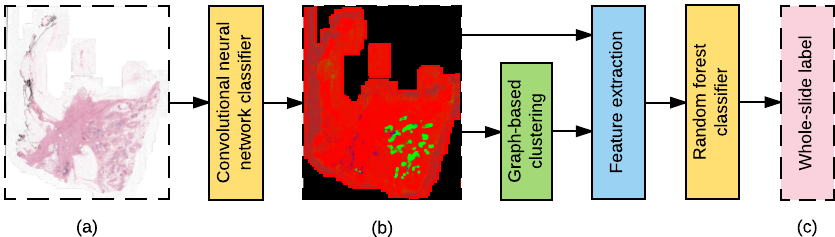
\includegraphics[width=6.5in]{system_overview}%
%\label{fig_first_case}}
%\hfil
%\subfloat[Case II]{\includegraphics[width=2.5in]{box}%
%\label{fig_second_case}}
\caption{Overview of the proposed system for labeling whole-slide images. (a) Original WSI of breast tissue. (b) Resulting probability map of applying the CNN in a patch-based fashion. (c) Output of the system; a single label for the whole-slide image (either benign, DCIS or IDC).}
\end{figure*}




TODO more about domain, dataset


\section{Dense prediction}

TODO a lot
\subsection{Architectures}

We will apply two different architectures to the problem of patch classification, with patches of size 224x224 pixels.


\subsubsection{Wide Residual Networks}
Residual network was the winner of the 2015 ImageNet challenge \cite{resnet}. Other than previous networks that entered this competition, it features no fully connected layer at the end of the network. It was the deepest succesful architecture to date featuring up to 152 layers. It can get away with this depth by using residual learning blocks, where the layers learn residual functions with relation to the input instead of learning unreferenced functions. To the extreme, it makes it easier to learn the identity function if that is optimal for that layer.

In this study we will apply an adaptation of this architecture, the wide residual network as proposed by Zagoruyko et al. \cite{wideresnet}. They showed that wider and less deep residual networks outperform their deeper and thinner counterparts both in accuracy and efficiency. 

The architecture is a recipe that has three main design choices, the $N$ value that determines the depth, the $k$ value that determines the width (the amount of filters) and the type of ResNet block. Here, we use $N=4$, $k=2$, which was empirically evaluated to fit a decent batch size and train fast. The ResNet block type is detailed in figure \ref{fig_resnet_block}, TODO more about this block. The resulting architecture is shown in figure \ref{fig_resnet}.

\subsubsection{VGG-16}
VGG-16 is a popular architecture because of its simplicity. It features small 3x3 convolution filters and 2x2 pooling throughout the network and has a depth of 16 layers. The architecture is detailed in figure \ref{fig_vgg}. Unlike the ResNet architecture it does not feature skip connections, also it features a stack of two dense fully connected layers at the end.


\begin{figure*}[!t]
\centering
\subfloat[{Wide Residual Network architecture. \newline \emph{RB} stands for ResNet Block.}]{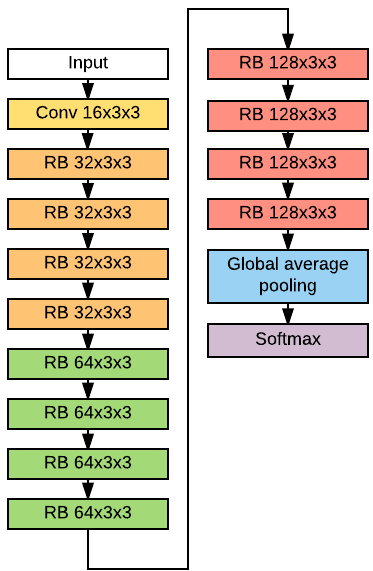
\includegraphics[width=2.20in]{architecture_wide_resnet}%
\label{fig_resnet}}
\subfloat[{Architecture of the resnet blocks. \newline The $\otimes$ node indicates an elementwise sum.}]{\hspace{0.8cm}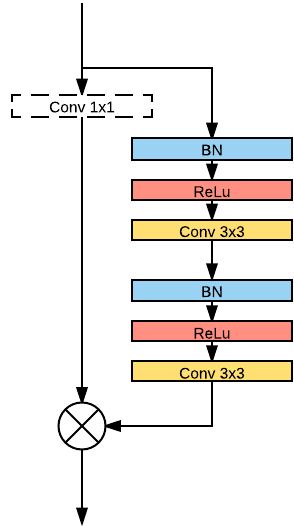
\includegraphics[width=1.8in]{architecture_resnet_block}%
\label{fig_resnet_block}}
\subfloat[VGG-16 model architecture. \newline Dropout with probability of 0.5 was used in the fully connected layers.]{\hspace{0.98cm}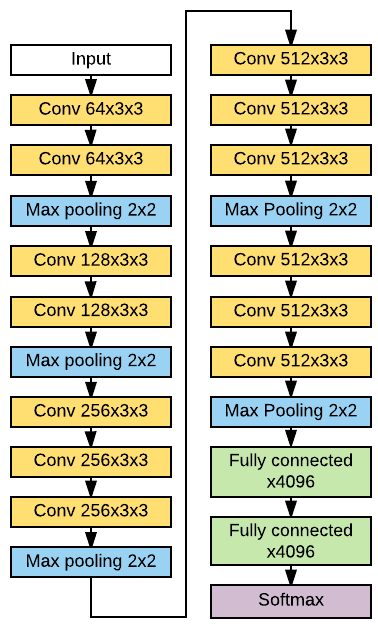
\includegraphics[width=2.20in]{architecture_vgg}%
\label{fig_vgg}}
\caption{Architectures used for 224x224 patch classification. The 1x1 convolution layer in the resnet blocks is only present in the blocks where the input is downsampled, which is every first block with a higher amount of filters in the Wide ResNet architecture (figure \ref{fig_resnet}).}
\label{fig_architectures}
\end{figure*}




\subsection{Preprocessing}
As a preprocessing step, the images are normalized by dividing their pixel value by 255. Then, the mean value of each color channel is subtracted to zero center the data.

\subsection{Learning rate decay}
The learning rate reduction policy is as follows. The learning rate is multiplied by 0.2 after no better validation accuracy has been observed for 8 epochs, this value is called the \emph{patience}. This patience is increased by 20\% after every reduction in learning rate (rounded up).  

\subsection{Data augmentation}
Artificially increasing the amount of data by adding variations of the original data can further help train a model that generalizes well. Augmentation consists of applying (random) pertubations to the samples in ways that do not change the label of the samples. It has a regularizing effect which helps prevent overfitting. Especially effective are augmentations that are also realistic examples of real world data.

\medskip

The augmentation methods used are as follows:

\subsubsection{Flips}
The images are randomly mirrored in the X and/or Y direction, both with a 0.5 probability. 

\subsubsection{Rotations}
The images are randomly rotated 0, 90, 180, or 270 degrees with equal probability.

\subsubsection{HSV jittering}
HSV is a colorspace that represents a color image in three channels; a \emph{hue} (color), \emph{saturation} (vibrance) and a \emph{value} (brightness) channel. There exists a large variability in the staining of the slides, which shows itself mostly in the hue and saturation channel. We randomly jitter the hue and saturation of an image with a random value between -0.075 and 0.075. The values of all pixels are then clipped between 0 and 1.

\medskip

Another commonly used data augmentation method is also zooming. This was not used here, as the size of the nuclei plays a role in determining the class label. Elastic distortions were succesfully applied as part of the data augmentation strategy in other applications of convolutional neural networks \cite{elastransforms}, also in the medical imaging domain (cytology) \cite{unet}. The irregularity of the sizes of the nuclei, as well as the architectural features are important biomarkers that can be used to distinguish between benign and cancerous lesions. Applying these elastic distortions would likely contaminate this information, and as such, it was not used here.




\begin{figure}[!t]
\centering{}
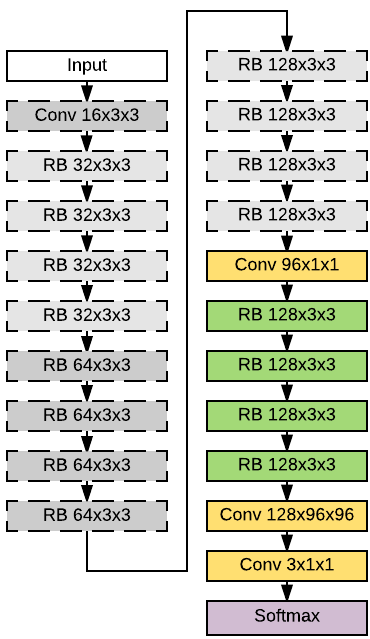
\includegraphics[width=2.5in]{architecture_stacked}
\caption{Architecture of the stacked network. The weights of the components with the dotted outlines are taken from the previously trained 224x224 patch model, and are no longer updated (these are frozen).}
\label{fig_stacked}
\end{figure}





% An example of a floating figure using the graphicx package.
% Note that \label must occur AFTER (or within) \caption.
% For figures, \caption should occur after the \includegraphics.
% Note that IEEEtran v1.7 and later has special internal code that
% is designed to preserve the operation of \label within \caption
% even when the captionsoff option is in effect. However, because
% of issues like this, it may be the safest practice to put all your
% \label just after \caption rather than within \caption{}.
%
% Reminder: the "draftcls" or "draftclsnofoot", not "draft", class
% option should be used if it is desired that the figures are to be
% displayed while in draft mode.
%
%\begin{figure}[!t]
%\centering
%\includegraphics[width=2.5in]{myfigure}
% where an .eps filename suffix will be assumed under latex, 
% and a .pdf suffix will be assumed for pdflatex; or what has been declared
% via \DeclareGraphicsExtensions.
%\caption{Simulation results for the network.}
%\label{fig_sim}
%\end{figure}

% Note that the IEEE typically puts floats only at the top, even when this
% results in a large percentage of a column being occupied by floats.


% An example of a double column floating figure using two subfigures.
% (The subfig.sty package must be loaded for this to work.)
% The subfigure \label commands are set within each subfloat command,
% and the \label for the overall figure must come after \caption.
% \hfil is used as a separator to get equal spacing.
% Watch out that the combined width of all the subfigures on a 
% line do not exceed the text width or a line break will occur.
%
%\begin{figure*}[!t]
%\centering
%\subfloat[Case I]{\includegraphics[width=2.5in]{box}%
%\label{fig_first_case}}
%\hfil
%\subfloat[Case II]{\includegraphics[width=2.5in]{box}%
%\label{fig_second_case}}
%\caption{Simulation results for the network.}
%\label{fig_sim}
%\end{figure*}
%
% Note that often IEEE papers with subfigures do not employ subfigure
% captions (using the optional argument to \subfloat[]), but instead will
% reference/describe all of them (a), (b), etc., within the main caption.
% Be aware that for subfig.sty to generate the (a), (b), etc., subfigure
% labels, the optional argument to \subfloat must be present. If a
% subcaption is not desired, just leave its contents blank,
% e.g., \subfloat[].


% An example of a floating table. Note that, for IEEE style tables, the
% \caption command should come BEFORE the table and, given that table
% captions serve much like titles, are usually capitalized except for words
% such as a, an, and, as, at, but, by, for, in, nor, of, on, or, the, to
% and up, which are usually not capitalized unless they are the first or
% last word of the caption. Table text will default to \footnotesize as
% the IEEE normally uses this smaller font for tables.
% The \label must come after \caption as always.
%
%\begin{table}[!t]
%% increase table row spacing, adjust to taste
%\renewcommand{\arraystretch}{1.3}
% if using array.sty, it might be a good idea to tweak the value of
% \extrarowheight as needed to properly center the text within the cells
%\caption{An Example of a Table}
%\label{table_example}
%\centering
%% Some packages, such as MDW tools, offer better commands for making tables
%% than the plain LaTeX2e tabular which is used here.
%\begin{tabular}{|c||c|}
%\hline
%One & Two\\
%\hline
%Three & Four\\
%\hline
%\end{tabular}
%\end{table}


% Note that the IEEE does not put floats in the very first column
% - or typically anywhere on the first page for that matter. Also,
% in-text middle ("here") positioning is typically not used, but it
% is allowed and encouraged for Computer Society conferences (but
% not Computer Society journals). Most IEEE journals/conferences use
% top floats exclusively. 
% Note that, LaTeX2e, unlike IEEE journals/conferences, places
% footnotes above bottom floats. This can be corrected via the
% \fnbelowfloat command of the stfloats package.


\section{Whole-slide image labeling}

\section{Results}

\begin{figure}[!t]
\centering{}
\hspace{-0.3cm}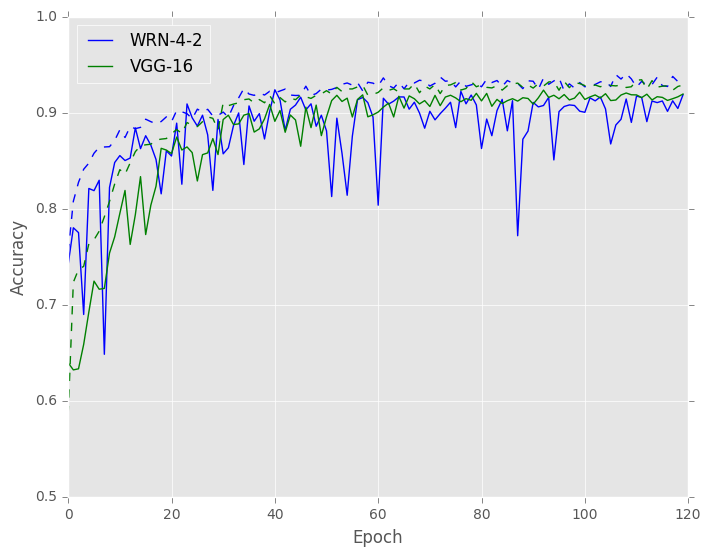
\includegraphics[width=3.5in]{2class_performance}
\caption{Performance of networks trained on the two class problem of benign versus cancerous patches. The dashed line shows the performance on the images from the train set it was shown that epoch.}
\label{fig_2class}
\end{figure}

\begin{figure}[!t]
\centering{}
\hspace{-0.3cm}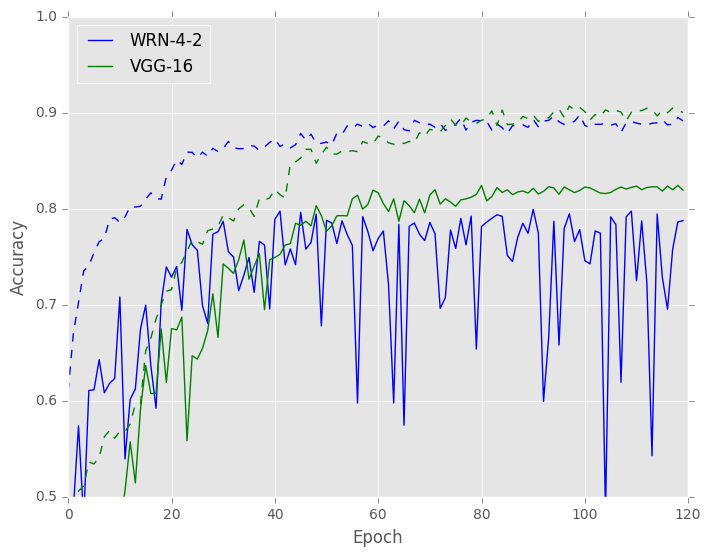
\includegraphics[width=3.5in]{3class_performance}
\caption{Performance of networks trained on all three classes. The dashed line shows the performance on the images from the train set it was shown that epoch. The validation accuracy of the wide resnet is especially noisy.}
\label{fig_3class}
\end{figure}



\begin{table}[h]
%% increase table row spacing, adjust to taste
\renewcommand{\arraystretch}{1.1}
% if using array.sty, it might be a good idea to tweak the value of
% \extrarowheight as needed to properly center the text within the cells
\caption{Best epoch patch-level accuracy of 224x224 networks}
\label{table_results_224}
\centering
%% Some packages, such as MDW tools, offer better commands for making tables
%% than the plain LaTeX2e tabular which is used here.
\begin{tabular}{|llr|}
\hline
\textsc{Labels}&\textsc{Architecture}&\textsc{Accuracy}\\
\hline
\textit{Benign, Cancer}&&\\
&VGG-16&  0.9237\\
&WRN-4-2& 0.9241\\
\hline
\textit{Benign, DCIS, IDC}&&\\
&VGG-16& 0.8245\\
&WRN-4-2& 0.7995\\
\hline
\end{tabular}
\end{table}




\begin{table}[!t]
%% increase table row spacing, adjust to taste
\renewcommand{\arraystretch}{1.1}
% if using array.sty, it might be a good idea to tweak the value of
% \extrarowheight as needed to properly center the text within the cells
\caption{Best epoch patch-level accuracy of 768x768 stacked networks}
\label{table_results_stacked}
\centering
%% Some packages, such as MDW tools, offer better commands for making tables
%% than the plain LaTeX2e tabular which is used here.
\begin{tabular}{|llr|}
\hline
\textsc{Labels}&\textsc{Stacked on}&\textsc{Accuracy}\\
\hline
\textit{Benign, Cancer}&&\\
&2 Class WRN-4-2&  123\\
&3 Class WRN-4-2& 123\\
\hline
\textit{Benign, DCIS, IDC}&&\\
&2 Class WRN-4-2&  123\\
&3 Class WRN-4-2& 123\\
\hline
\end{tabular}
\end{table}




\section{Conclusion}
The conclusion goes here.





% if have a single appendix:
%\appendix[Proof of the Zonklar Equations]
% or
%\appendix  % for no appendix heading
% do not use \section anymore after \appendix, only \section*
% is possibly needed

% use appendices with more than one appendix
% then use \section to start each appendix
% you must declare a \section before using any
% \subsection or using \label (\appendices by itself
% starts a section numbered zero.)
%


%\appendices
%\section{Proof of the First Zonklar Equation}
%Appendix one text goes here.

% you can choose not to have a title for an appendix
% if you want by leaving the argument blank
%\section{}
%Appendix two text goes here.


% use section* for acknowledgment
\section*{Acknowledgment}


The authors would like to thank...


% Can use something like this to put references on a page
% by themselves when using endfloat and the captionsoff option.
\ifCLASSOPTIONcaptionsoff
  \newpage
\fi



% trigger a \newpage just before the given reference
% number - used to balance the columns on the last page
% adjust value as needed - may need to be readjusted if
% the document is modified later
%\IEEEtriggeratref{8}
% The "triggered" command can be changed if desired:
%\IEEEtriggercmd{\enlargethispage{-5in}}

% references section

% can use a bibliography generated by BibTeX as a .bbl file
% BibTeX documentation can be easily obtained at:
% http://mirror.ctan.org/biblio/bibtex/contrib/doc/
% The IEEEtran BibTeX style support page is at:
% http://www.michaelshell.org/tex/ieeetran/bibtex/
\bibliographystyle{IEEEtran}
% argument is your BibTeX string definitions and bibliography database(s)
\bibliography{IEEEabrv,bib/ref}
%,
% <OR> manually copy in the resultant .bbl file
% set second argument of \begin ,to the number of references
% (used to reserve space for the reference number labe,ls box)
%\begin{thebibliography}{1}

%\bibitem{IEEEhowto:kopka}
%H.~Kopka and P.~W. Daly, \emph{A Guide to \LaTeX}, 3rd~ed.\hskip 1em plus
%  0.5em minus 0.4em\relax Harlow, England: Addison-Wesley, 1999.

%\end{thebibliography}

% biography section
% 
% If you have an EPS/PDF photo (graphicx package needed) extra braces are
% needed around the contents of the optional argument to biography to prevent
% the LaTeX parser from getting confused when it sees the complicated
% \includegraphics command within an optional argument. (You could create
% your own custom macro containing the \includegraphics command to make things
% simpler here.)
%\begin{IEEEbiography}[{\includegraphics[width=1in,height=1.25in,clip,keepaspectratio]{mshell}}]{Michael Shell}
% or if you just want to reserve a space for a photo:

%\begin{IEEEbiography}{Michael Shell}
%Biography text here.
%\end{IEEEbiography}

% if you will not have a photo at all:
%\begin{IEEEbiographynophoto}{John Doe}
%Biography text here.
%\end{IEEEbiographynophoto}

% insert where needed to balance the two columns on the last page with
% biographies
%\newpage

%\begin{IEEEbiographynophoto}{Jane Doe}
%Biography text here.
%\end{IEEEbiographynophoto}

% You can push biographies down or up by placing
% a \vfill before or after them. The appropriate
% use of \vfill depends on what kind of text is
% on the last page and whether or not the columns
% are being equalized.

%\vfill

% Can be used to pull up biographies so that the bottom of the last one
% is flush with the other column.
%\enlargethispage{-5in}



% that's all folks
\end{document}


